%%=============================================================================
%% demo.tex for Xiamen University Graduate Thesis
%% modified by Maozhong Fu
%% Version: 1.0
%% Last update: 2020/09/30
%% Based on BIT-thesis at https://github.com/BIT-thesis/LaTeX-template
%%==============================================================================

% 默认单面打印 oneside 、硕士论文模板 master

\documentclass[twoside, doctor]{xmu-thesis-grd}

% 模板选项: 硕士论文 master; 博士论文 doctor

%==============更改数学字体设置,Latin Modern Math 默认的的确有点细,看个人需要,下面提供一种方法,需要的可以取消注释=========%

% \usepackage[bold-style=ISO]{unicode-math} %采用unicode-math,可以直接输入Unicode公式,当然传统的输入就行
% \setmathfont{XITS Math}  %目前unicode-math 支持几种数学字体,具体用法可以查看帮助文档,这里采用类似times字体科学数学字体,可以取消注释对比


\begin{document}

%%%%%%%%%%%%%%%%%%%%%%%%%%%%%%
%% 封面
%%%%%%%%%%%%%%%%%%%%%%%%%%%%%%

% 中文封面内容(关注内容而不是表现形式)
\title{资产重组:一个资不抵债国有企业的最佳选择}
\author{某某某}
\advisor{某某某教授}
\major{信息与信号处理}
\submitdate{2021年6月}
\defenddate{2021年6月}
\grantdate{2021年6月}
\printdate{2021年6月}
%\studentnumber{**********}

% 封面
\makecover

% 学位论文原创性声明
\makeoriginalitystatement

% 学位论文著作权使用声明
\makecopyrightstatement

%%%%%%%%%%%%%%%%%%%%%%%%%%%%%%
%% 前置部分
%%%%%%%%%%%%%%%%%%%%%%%%%%%%%%
\frontmatter

% 摘要
%%==================================================
%% abstract.tex for BIT Master Thesis
%% modified by yang yating
%% version: 0.1
%% last update: Dec 25th, 2016
%%==================================================

\begin{abstract}
本文……。({\color{blue}{摘要是一篇具有独立性和完整性的短文,应概括而扼要地反映出本论文的主要内容。包括研究目的、研究方法、研究结果和结论等,特别要突出研究结果和结论。中文摘要力求语言精炼准确,硕士学位论文摘要建议500$\sim$800字,博士学位论文建议1000$\sim$1200字。摘要中不可出现参考文献、图、表、化学结构式、非公知公用的符号和术语。英文摘要与中文摘要的内容应一致。}})

\keywords{形状记忆; 聚氨酯; 织物; 合成; 应用 ({\color{blue}{一般选3~8个单词或专业术语,且中英文关键词必须对应。})}}
\end{abstract}

\begin{enabstract}

   In order to exploit …….
   
\enkeywords{shape memory properties; polyurethane; textile; synthesis; application}

\end{enabstract}


%% 符号对照表,可选,如不用可注释掉
\begin{notations}
\item[XMU] 厦门大学的英文缩写
\item[\LaTeX] 一个很棒的排版系统
\item[\LaTeXe] 一个很棒的排版系统的最新稳定版
\item[\XeTeX] \LaTeX{}的好兄弟,事实上他有很多个兄弟,但是这个兄弟对各种语言的支持能力都很强
\item[ctex] 成套的中文\LaTeX{}解决方案,由一帮天才们开发
\item[\ce{H2SO4}] 硫酸
\item[$ e^{\pi{}i}+1=0$] 一个集自然界五大常数一体的炫酷方程
\item[\ce{2H2 + O2 -> 2H2O}] 一个昂贵的生成生命之源的方程式
\end{notations}


% 加入目录
\tableofcontents
\entableofcontents

%加入图、表索引(同时取消图表索引中章之间的垂直间隔)
\makelistoffigures
\makelistoftables

%%%%%%%%%%%%%%%%%%%%%%%%%%%%%%
%% 正主体部分
%%%%%%%%%%%%%%%%%%%%%%%%%%%%%%
\mainmatter
%%==================================================
%% chapter01.tex for BIT Master Thesis
%% modified by yang yating
%% version: 0.1
%% last update: Dec 25th, 2016
%%==================================================
\chapter{绪论}
\enchapter{Introduction}
\label{chap:intro}
\section{研究背景及选题意义}
\ensection{Research Background and Motivation}
近年来,随着人们生活水平的不断提高,人们越来越注重周围环境对身体健康的影响。作为服装是人们时时刻刻最贴近的环境,尤其是内衣,对人体健康有很大的影响。由于合时刻刻最贴近的环境,尤其是内衣,对人体健康有很大的影响。由于合成纤维的衣着舒适性、手感性,天然纤维的发展又成为人们关注的一大热点。

\upcite{Takahashi1996Structure,Xia2002Analysis,Jiang1989,Mao2000Motion,Feng1998}

\section{国内外研究现状}
\ensection{Research Progress Overview in Home and Abroad}
%\label{sec:***} 可标注label

\section{本文主要内容和章节安排}
\ensection{Major Contents and Chapter Arrangement}

%\label{sec:features}

形状记忆聚合物(SMP)是继形状记忆合金后在80年代发展起来的一种新型形状记忆材料\cite{Jiang2005Size}。形状记忆高分子材料在常温范围内具有塑料的性质,即刚性、形状稳定恢复性;同时在一定温度下(所谓记忆温度下)具有橡胶的特性,主要表现为材料的可变形性和形变恢复性。即“记忆初始态-固定变形-恢复起始态”的循环。

固定相只有物理交联结构的聚氨酯称为热塑性SMPU,而有化学交联结构称为热固性SMPU。热塑性和热固性形状记忆聚氨酯的形状记忆原理示意图如图\ref{fig:diagram}所示

\begin{figure}
 \centering
 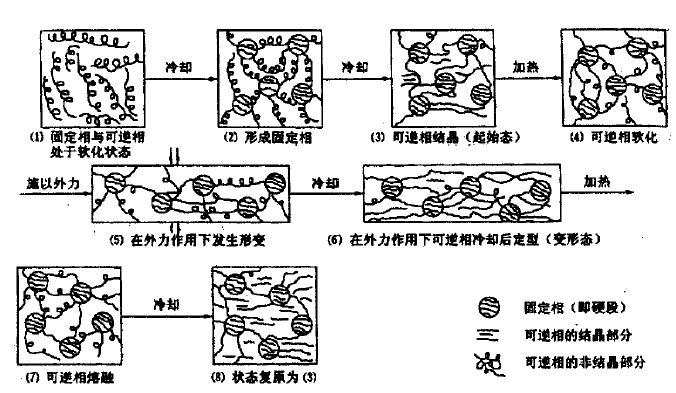
\includegraphics[width=0.75\textwidth]{figures/figure1}
 \caption{热塑性形状记忆聚氨酯的形状记忆机理示意图}\label{fig:diagram}
\end{figure}


\subsection{形状记忆聚氨酯的研究进展}
%\label{sec:requirements}
首例SMPU是日本Mitsubishi公司开发成功的……。

\subsection{水系聚氨酯及聚氨酯整理剂}

水系聚氨酯的形态对其流动性,成膜性及加工织物的性能有重要影响,一般分为三种类型\cite{Jiang2005Size} ,如表 \ref{tab:category}所示。

\begin{table}
  \centering
  \caption{水系聚氨酯分类} \label{tab:category}
  \begin{tabular*}{0.9\textwidth}{@{\extracolsep{\fill}}cccc}
  \toprule
    类别			&水溶型		&胶体分散型		&乳液型 \\
  \midrule
    状态			&溶解$\sim$胶束	&分散		&白浊 \\
    外观			&水溶型		&胶体分散型		&乳液型 \\
    粒径$/\mu m$	&$<0.001$		&$0.001-0.1$		&$>0.1$ \\
    重均分子量	&$1000\sim 10000$	&数千$\sim 20万$ &$>5000$ \\
  \bottomrule
  \end{tabular*}
\end{table}

由于它们对纤维织物的浸透性和亲和性不同,因此在纺织品染整加工中的用途也有差别,其中以水溶型和乳液型产品较为常用。另外,水系聚氨酯又有反应性和非反应性之分。虽然它们的共同特点是分子结构中不含异氰酸酯基,但前者是用封闭剂将异氰酸酯基暂时封闭,在纺织品整理时复出。相互交联反应形成三维网状结构而固着在织物表面。
……


%\include{chapters/chapter2}
%\include{chapters/chapter3}

%%==================================================
%% conclusion.tex for BIT Master Thesis
%% modified by yang yating
%% version: 0.1
%% last update: Dec 25th, 2016
%%==================================================
\chapter{总结与展望}
\label{chap:conlution}
本文采用……。{\color{blue}(结论作为学位论文正文的最后部分单独排写,但不加章号。结论是对整个论文主要结果的总结。在结论中应明确指出本研究的创新点,对其应用前景和社会、经济价值等加以预测和评价,并指出今后进一步在本研究方向进行研究工作的展望与设想。结论部分的撰写应简明扼要,突出创新性。)}


%% 参考文献,五号字,使用 BibTeX,包含参考文献文件.bib

%\bibliography{reference/chap1,reference/chap2} %多个章节的参考文献
\bibliography{reference/chapter1}

%%%%%%%%%%%%%%%%%%%%%%%%%%%%%%
%% 后置部分
%%%%%%%%%%%%%%%%%%%%%%%%%%%%%%

%% 附录(章节编号重新计算,使用字母进行编号)
\appendix
\setappendixnumberformat

%%==================================================
%% app1.tex for BIT Master Thesis
%% modified by yang yating
%% version: 0.1
%% last update: Dec 25th, 2016
%%==================================================


\chapter{关于XXX的证明}

附录相关内容…


\chapter{Maxwell Equations}


因为在柱坐标系下,$\overline{\overline\mu}$是对角的,所以Maxwell方程组中电场$\bf
E$的旋度

所以$\bf H$的各个分量可以写为:
\begin{subequations}
  \begin{eqnarray}
    H_r=\frac{1}{\mathbf{i}\omega\mu_r}\frac{1}{r}\frac{\partial
      E_z}{\partial\theta } \\
    H_\theta=-\frac{1}{\mathbf{i}\omega\mu_\theta}\frac{\partial E_z}{\partial r}
  \end{eqnarray}
\end{subequations}
同样地,在柱坐标系下,$\overline{\overline\epsilon}$是对角的,所以Maxwell方程组中磁场$\bf
H$的旋度
\begin{subequations}
  \begin{eqnarray}
    &&\nabla\times{\bf H}=-\mathbf{i}\omega{\bf D}\\
    &&\left[\frac{1}{r}\frac{\partial}{\partial
        r}(rH_\theta)-\frac{1}{r}\frac{\partial
        H_r}{\partial\theta}\right]{\hat{\bf
        z}}=-\mathbf{i}\omega{\overline{\overline\epsilon}}{\bf
      E}=-\mathbf{i}\omega\epsilon_zE_z{\hat{\bf z}} \\
    &&\frac{1}{r}\frac{\partial}{\partial
      r}(rH_\theta)-\frac{1}{r}\frac{\partial
      H_r}{\partial\theta}=-\mathbf{i}\omega\epsilon_zE_z
  \end{eqnarray}
\end{subequations}
由此我们可以得到关于$E_z$的波函数方程:
\begin{eqnarray}
  \frac{1}{\mu_\theta\epsilon_z}\frac{1}{r}\frac{\partial}{\partial r}
  \left(r\frac{\partial E_z}{\partial r}\right)+
  \frac{1}{\mu_r\epsilon_z}\frac{1}{r^2}\frac{\partial^2E_z}{\partial\theta^2}
  +\omega^2 E_z=0
\end{eqnarray}


%(其后部分无编号)
\backmatter

% 发表文章目录
%%==================================================
%% pub.tex for BIT Master Thesis
%% modified by yang yating
%% version: 0.1
%% last update: Dec 25th, 2016
%%==================================================

\begin{publications}{99}

    \item\textsc{高凌}. {交联型与线形水性聚氨酯的形状记忆性能比较}[J].
      化工进展, 2006, 532-535.(核心期刊)
    
\end{publications}


% 致谢
%%==================================================
%% acknowledgement.tex for BIT Master Thesis
%% modified by yang yating
%% version: 0.1
%% last update: Dec 25th, 2016
%%==================================================

\begin{acknowledgements}

本论文的工作是在导师……。

\end{acknowledgements}


\end{document}
